\chapter{Методы формирования структур и моделирования} \label{chapter:methods}

В настоящее время существует ряд областей, требующих формирования трехмерных микро- и наноструктур (нанофотоника, микро- и нанофлюидика, МЭМС и др.). Существующие методы формирования имеют как свои характерные достоинства, так и недостатки.

\section{Методы формирования трехмерных микро- и наноструктур}

\subsection{Наноимпринтная литография}
Наноимпринтная литография (НИЛ) -- технология, предназначенная для переноса изображения наноструктуры или электронной схемы на полимерный материал путем прямого воздействия на него специальным штампом~\cite{NIL_1, NIL_2}. Существуют два основных метода НИЛ -- термическая и ультрафиолетовая (УФ). В термической НИЛ штамп вдавливается в полимер, нагретый до температур выше температуры стеклования, затем происходит его охлаждение и извлечение штампа. В ультрафиолетовой НИЛ штамп из материала, прозрачного в УФ области спектра, погружается в жидкий полимер, который отверждается под действием УФ излучения, после чего происходит извлечение штампа. Штамп обычно изготавливается из металла или кремния (для термической НИЛ) и полимеров или кварца (для УФ НИЛ) с помощью электронно-лучевой литографии. Учитывая прямой контакт штампа с основным материалом, а также масштаб печати 1:1, к штампу предъявляются повышенные требования по плоскопараллельности и бездефектности.  Перед проведением процесса НИЛ штамп покрывается специальным антиадгезионным покрытием, что позволяет избежать прилипания полимера к штампу при его отделении. Также после печати неизбежно остаётся тонкий остаточный слой полимера, который удаляют с помощью плазменного травления. Преимуществами НИЛ являются простота процесса (при наличии штампа), высокая производительность и возможность достижения высокого разрешения (менее 100 нм). К недостаткам этого метода относятся трудоемкость и дороговизна процесса изготовления штампа надлежащего качества, необходимость частого его обслуживания (удаления остатков основного материала), а также сложность совмещения штампа с низлежащим слоем. Несмотря на то, что технология НИЛ изначально создавалась как альтернатива фото- и электронно-лучевой литографии, она может применяется для получения трехмерных микро- и наноструктур, таких как фотонные кристаллы~\cite{NIL_nanophotonics}, микроканалы~\cite{NIL_microfluidics} и др.~\cite{NIL_3D_1, NIL_3D_2}

\begin{fig}{NIL}{NIL_white_bg}
	Схематическое изображение процессов термической и УФ НИЛ.
\end{fig}

\subsection{Двухфотонная лазерная литография}

Двухфотонная лазерная литография (ДЛЛ) — технология создания микро- и наноструктур, основанная на двухфотонном поглощении внутри фокального объёма лазерного излучения~\cite{Hohmann2015, Kawata2001}. Фотовозбуждение компонент литографической смол приводящее к ее отверждению, происходит лишь в окрестности перетяжки сфокусированного лазерного излучения благодаря нелинейному характеру поглощения. Процесс отверждения имеет пороговый характер, что позволяет регулировать размер отверждаемого объёма, изменяя дозу или плотность энергии поглощённого лазерного излучения. Последующее погружение смолы в растворитель приводит к удалению тех участков, которые не были подвергнуты воздействию излучения. В качестве источника излучения в ДЛЛ обычно используется фемптосекундный лазер, работающий в инфракрасном диапазоне, в качестве литографической смолы -- вещество, содержащее реакционно-способные олигомеры и фотоинициатор. При точной фокусировке ДЛЛ способна обеспечить разрешение менее 1 мкм. Поскольку в ДЛЛ положение центров отвреждения может задаваться произвольно, эта технология нашла применение для формирования трехмерных во многих областях -- микрофлюидике~\cite{TPL_microfluidics_1, TPL_microfluidics_2}, биологии и \break медицины~\cite{TPL_biology_1, TPL_biology_2}, оптике и нанофотонике \cite{TPL_optics, TPL_nanophotonics}, и др. При этом, силу своей природы, данная технология обладает низкой производительностью, что является ее главным недостатком.

\begin{figure}
	\centering
	\begin{subfigure}{.5\textwidth}
		\centering
		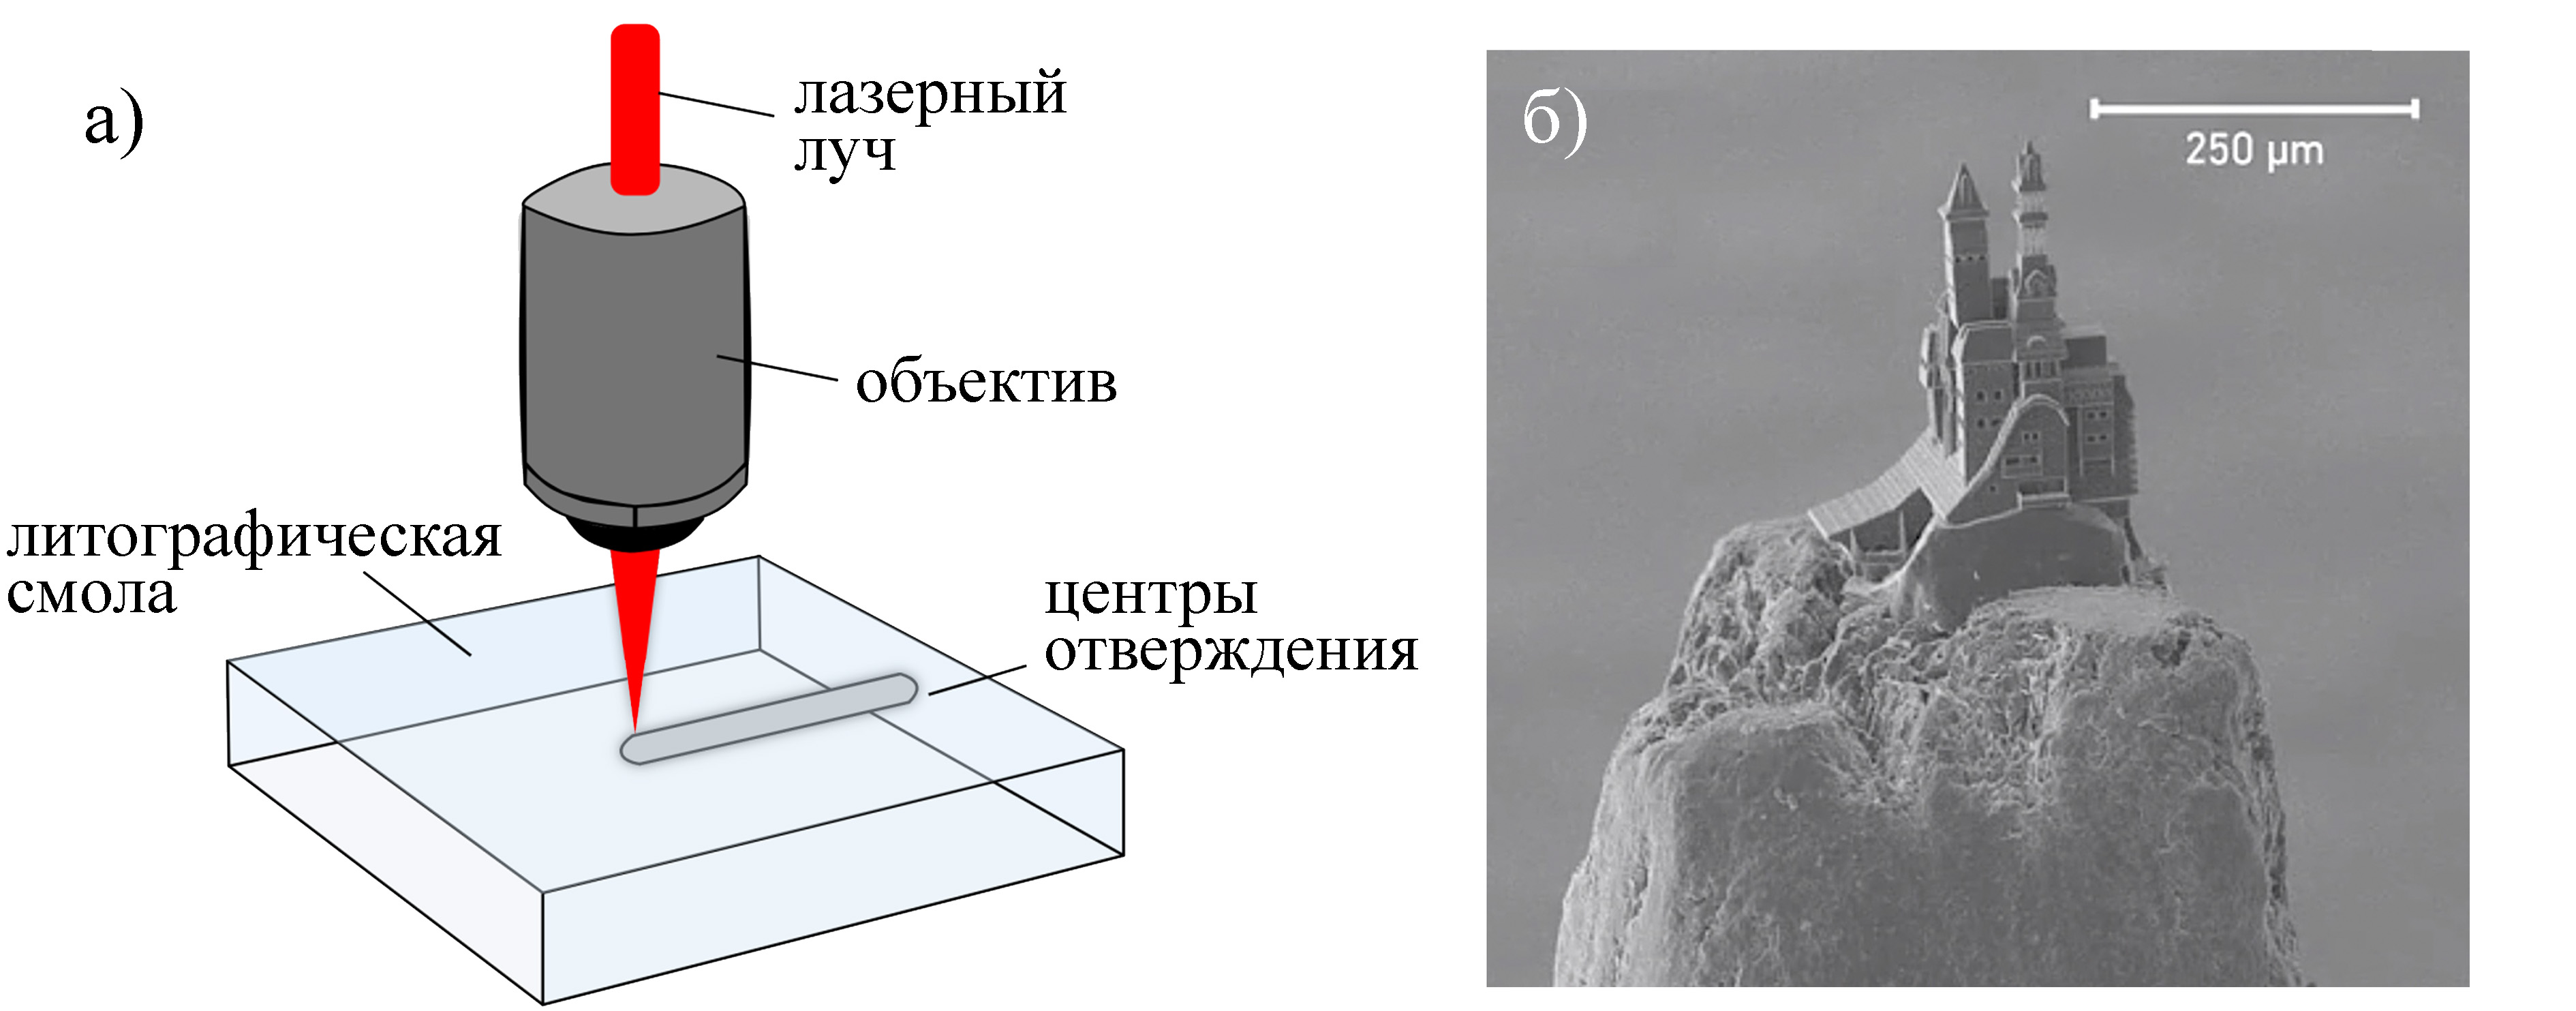
\includegraphics[width=.95\linewidth]{TPL}
	\end{subfigure}%
	\begin{subfigure}{.5\textwidth}
		\centering
		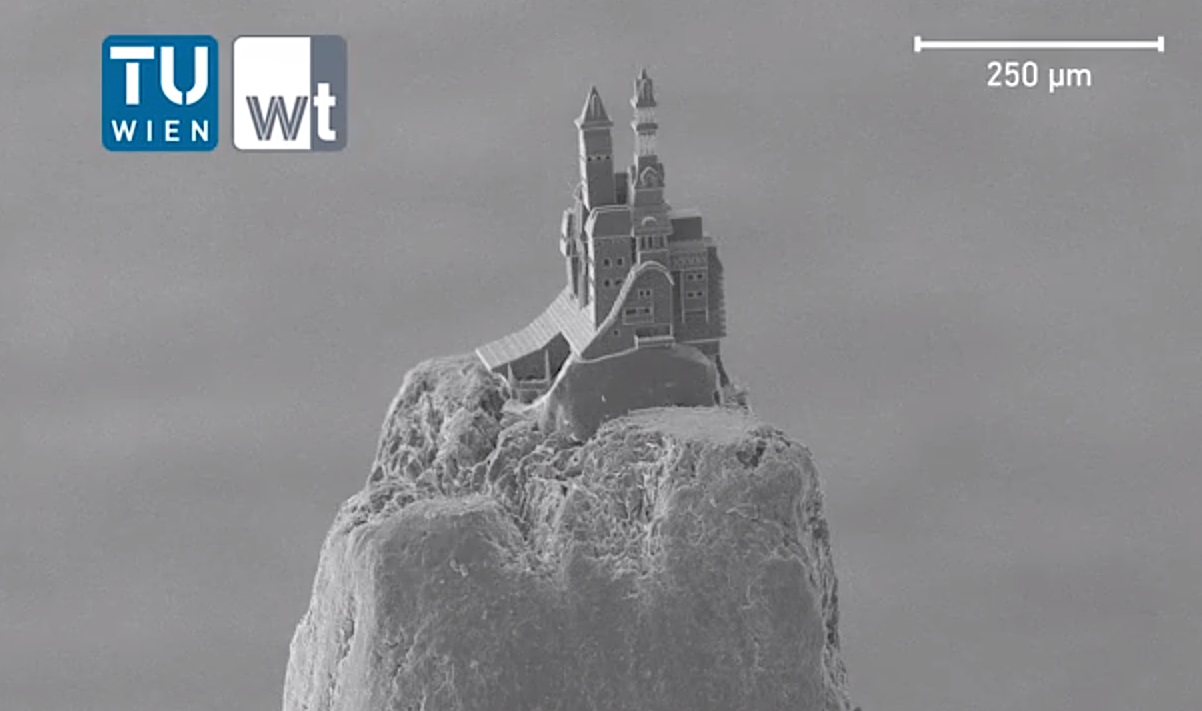
\includegraphics[width=.95\linewidth]{TPL_structure}
	\end{subfigure}
	\caption{Схематическое изображение процесса ДЛЛ и пример структуры.}
\end{figure}


\subsection{Интерференционная литография}

Интерференционная литография (ИЛ) -- метод формирования периодической структуры в резисте, основанный на экспонировании резиста пространственно упорядоченным стоячим электромагнитным полем, возникающим при интерференции двух и более когерентных монохроматических или квазимонохроматических пучков излучения~\cite{IL_general}. Когерентность интерферирующих пучков обычно обеспечивается путем разделения исходного когерентного пучка на соответствующее число пучков с помощью различных интерференционных схем. При наноструктурировании ИЛ применяется для получения  метаматериалов~\cite{IL_metamaterials}, нанофотонных и наноплазмонных устройств~\cite{IL_nanophotonics}, биомедицинских объектов~\cite{IL_biomedical}, изделий на основе выращиваемых наноэлементов и самоорганизующихся структур~\cite{IL_self-assembly} и др.
В оптическом и УФ-диапазонах используются зеркальные схемы (Френеля, Ллойда и др.), схемы на преломляющей оптике (бипризма Френеля, билинза Бийе) или комбинированные зеркально-линзовые схемы. В этих диапазонах в качестве источника исходного пучка с высокой степенью монохроматичности и когерентности используются мощные лазеры, позволяющие получить разрешение до 100 нм. Вопрос обеспечения высокого разрешения ИЛ решается путем перехода в область рентгеновского излучения~\cite{IL_X-ray}. К недостаткам метода можно отнести не самую высокую производительность и возможность получения исключительно периодических структур.

\begin{figure}
	\centering
	\begin{subfigure}{.5\textwidth}
		\centering
		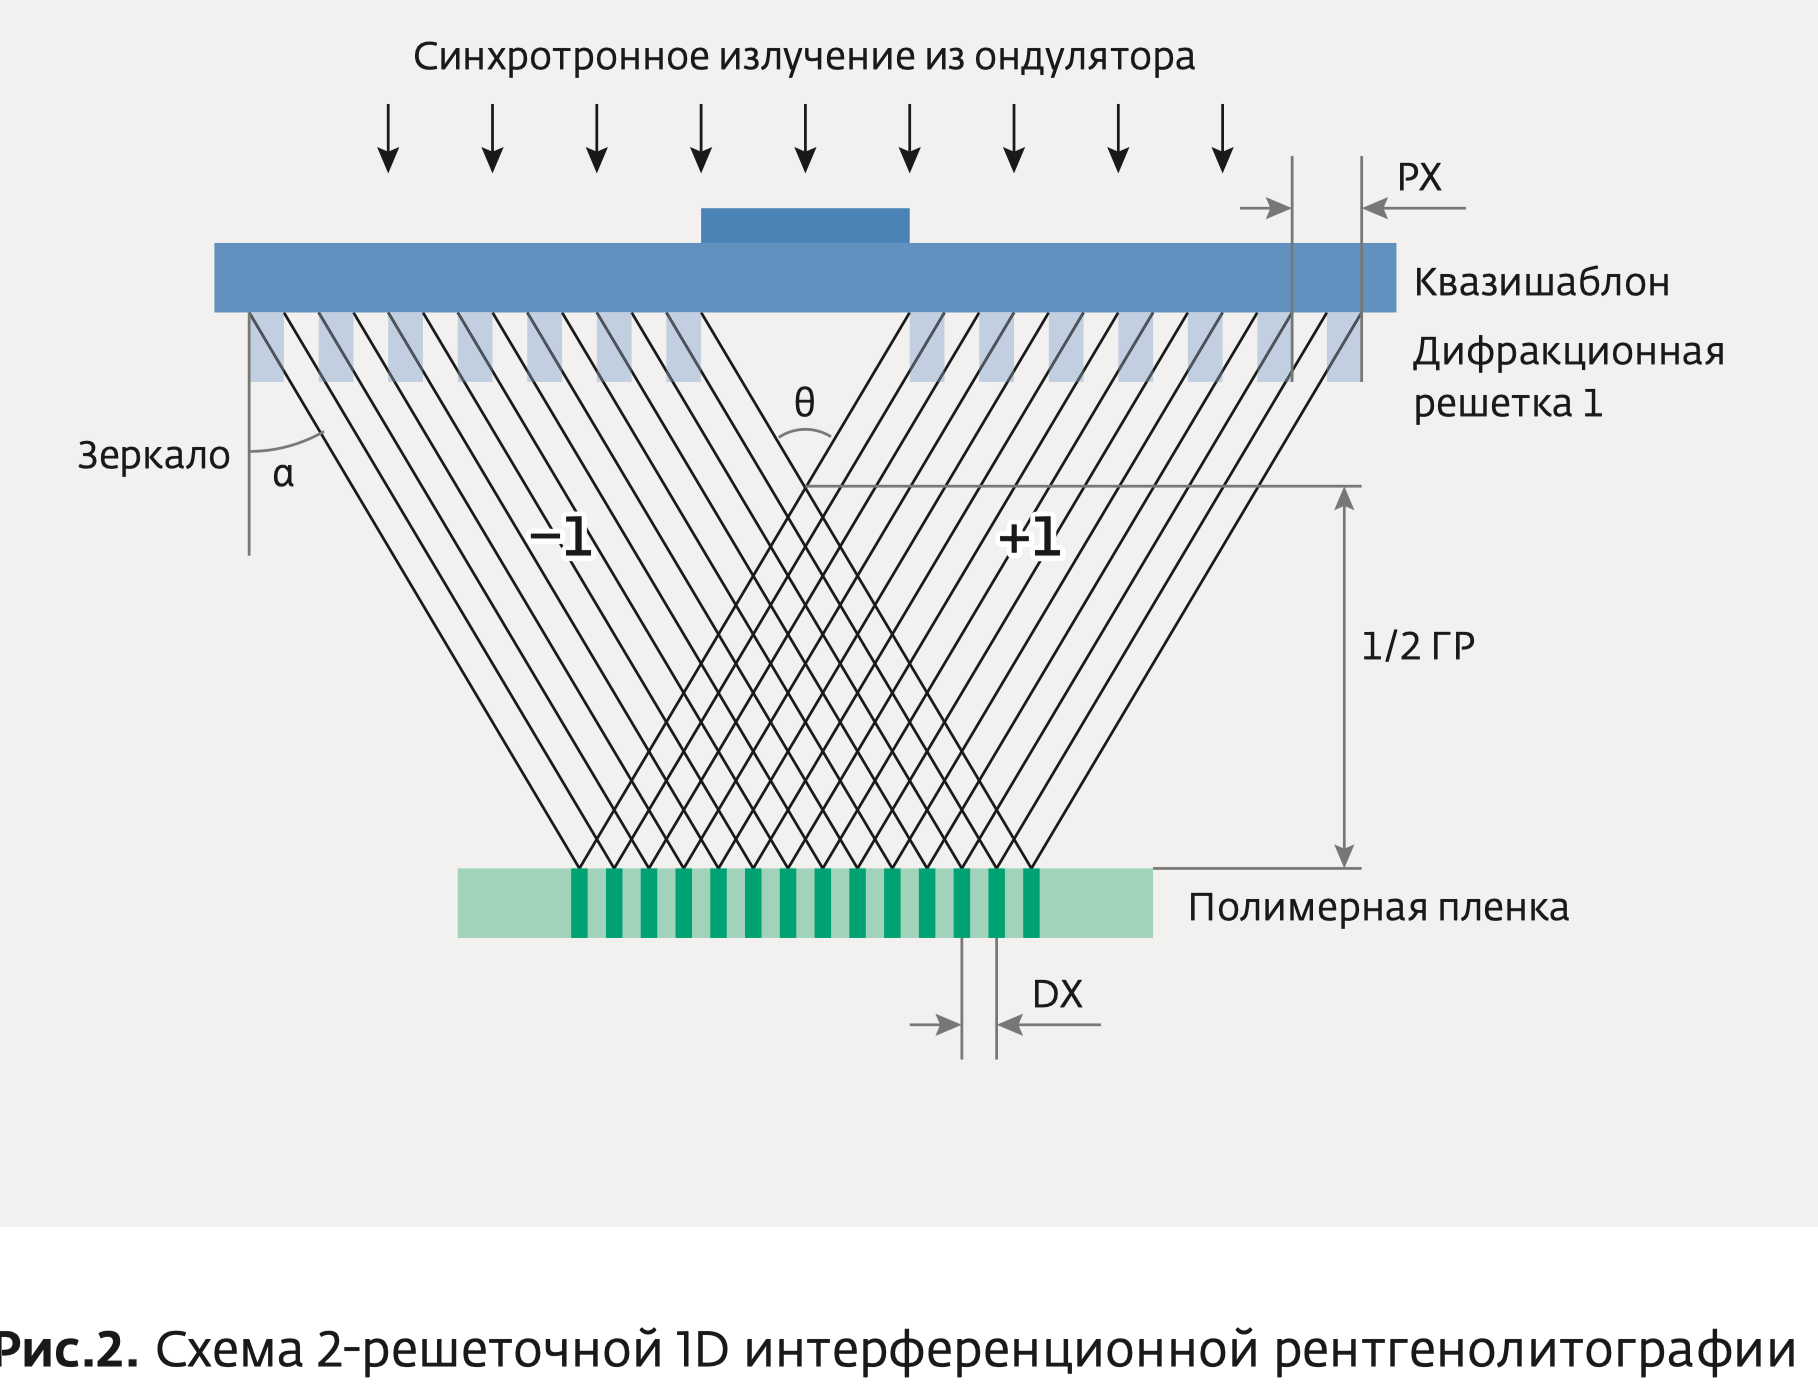
\includegraphics[width=.95\linewidth]{IL_1}
	\end{subfigure}%
	\begin{subfigure}{.5\textwidth}
		\centering
		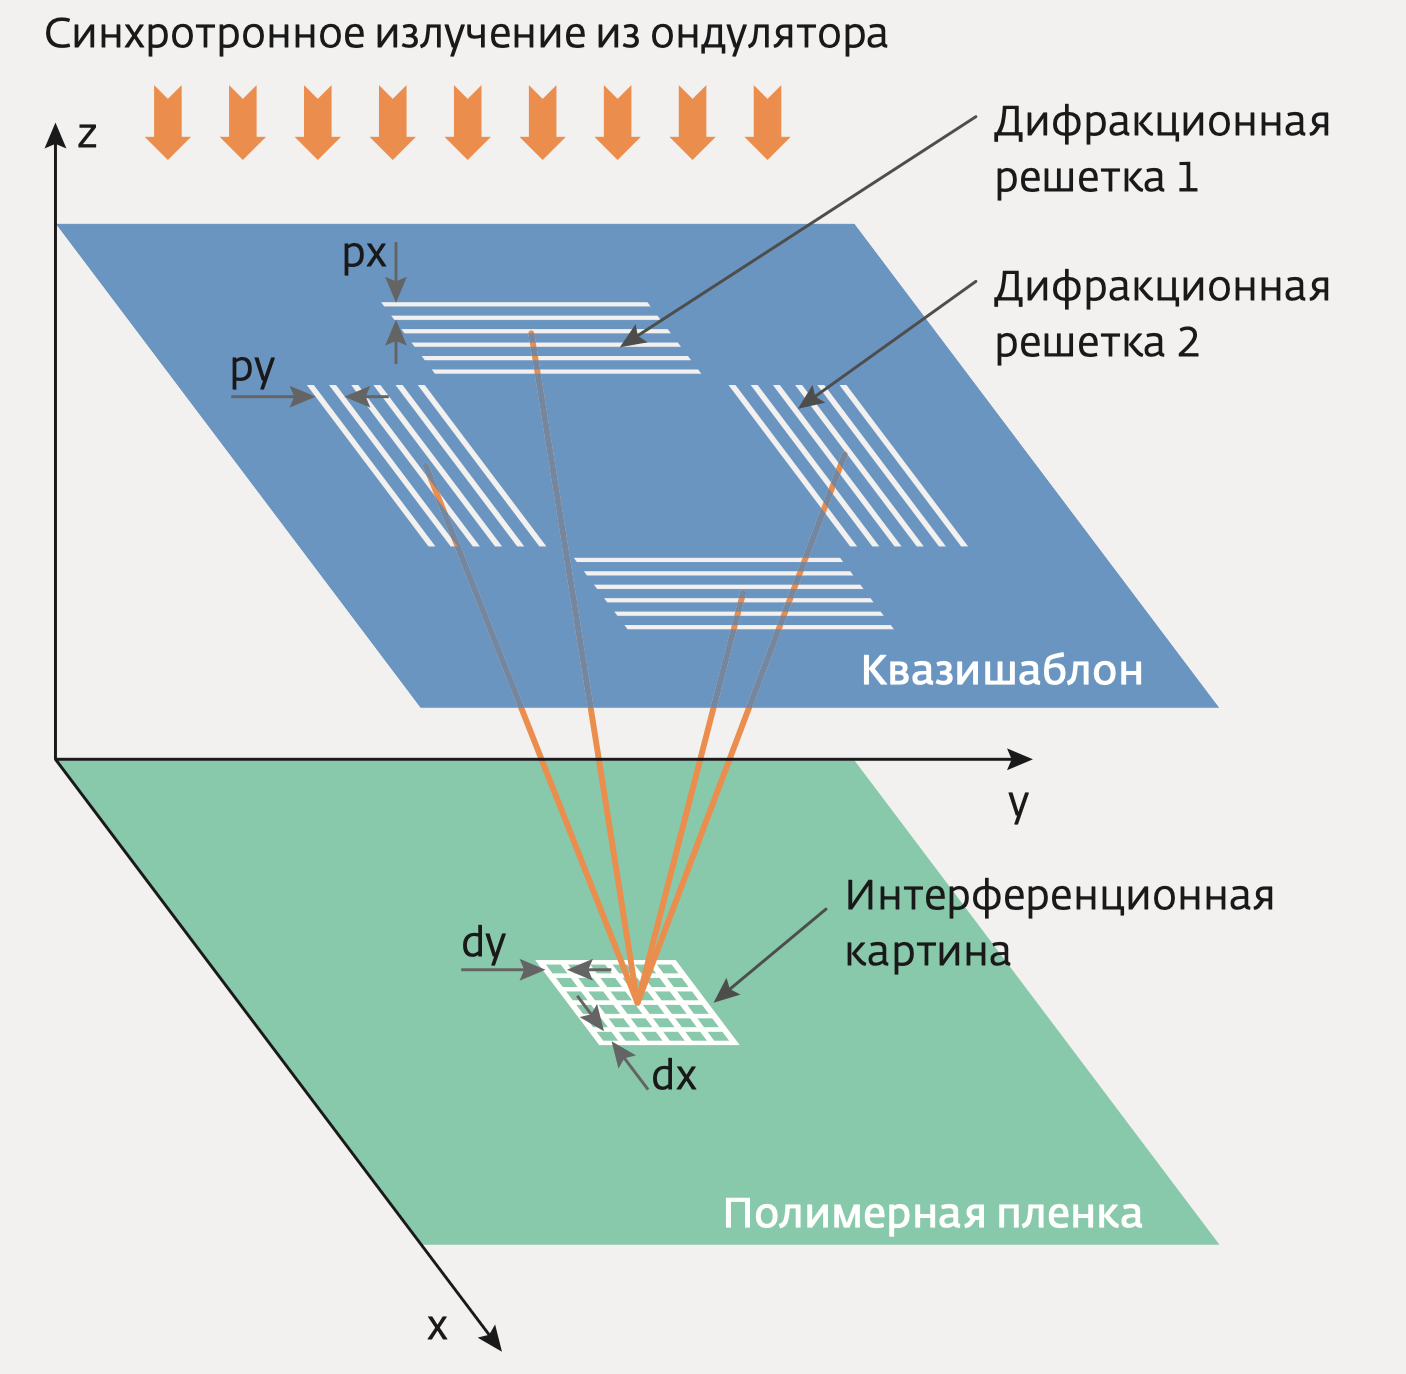
\includegraphics[width=.95\linewidth]{IL_2}
	\end{subfigure}
	\caption{Схематическое изображение процесса ИЛ.}
\end{figure}


\subsection{Полутоновая литография}

Полутоновая литография (ПЛ) -- общее название для методов, позволяющих получить сложный трехмерный рельеф в резисте в литографическом процессе с одной одной стадией экспонирования~\cite{GL_general}. В их основе лежит пространственная модуляция дозы при экспонировании, приводящая к локальному увеличению или уменьшению скорости растворения резиста при проявлении. Таким образом, конечный рельеф имеет ступенчатую форму и состоит из участков резиста, растворенных в различной степени. Сглаживание границы между участками, проэкспонированных с различными дозами, может быть в дальнейшем достигнуто за счет оплавления образца при температурах вблизи его температуры стеклования. При этом существующие методы моделирования эволюции поверхности полимеров при их оплавлении позволяют использовать этот процесс как дополнительный этап структурирования~\cite{Kirchner_reflow}. Таким образом, полутоновая литография с последующим оплавлением образца является гибкой технологией микро- и наноструктурирования, использующейся в оптике и нанофотонике~\cite{GL_optics}, микрофлюидике~\cite{GL_microfluidics}, формировании микроэлектромеханических систем~\cite{GL_MEMS} и других областях. Существует как электронно-лучевая, так и фото-ПЛ, однако, фото-ПЛ имеет некоторые ограничения, связанные с оплавлением резиста. Так, например, вязкость широко распространенного негативного фоторезиста SU-8 при экспонировании увеличивается, что усложняет процесс контролируемого оплавления~\cite{Kirchner_GL_review}. К недостаткам метода можно отнести его сложность и производительность, еще более низкую, чем при электронно-лучевой и фотолитографии за счет дополнительной стадии оплавления образца.

\begin{figure}
	\centering
	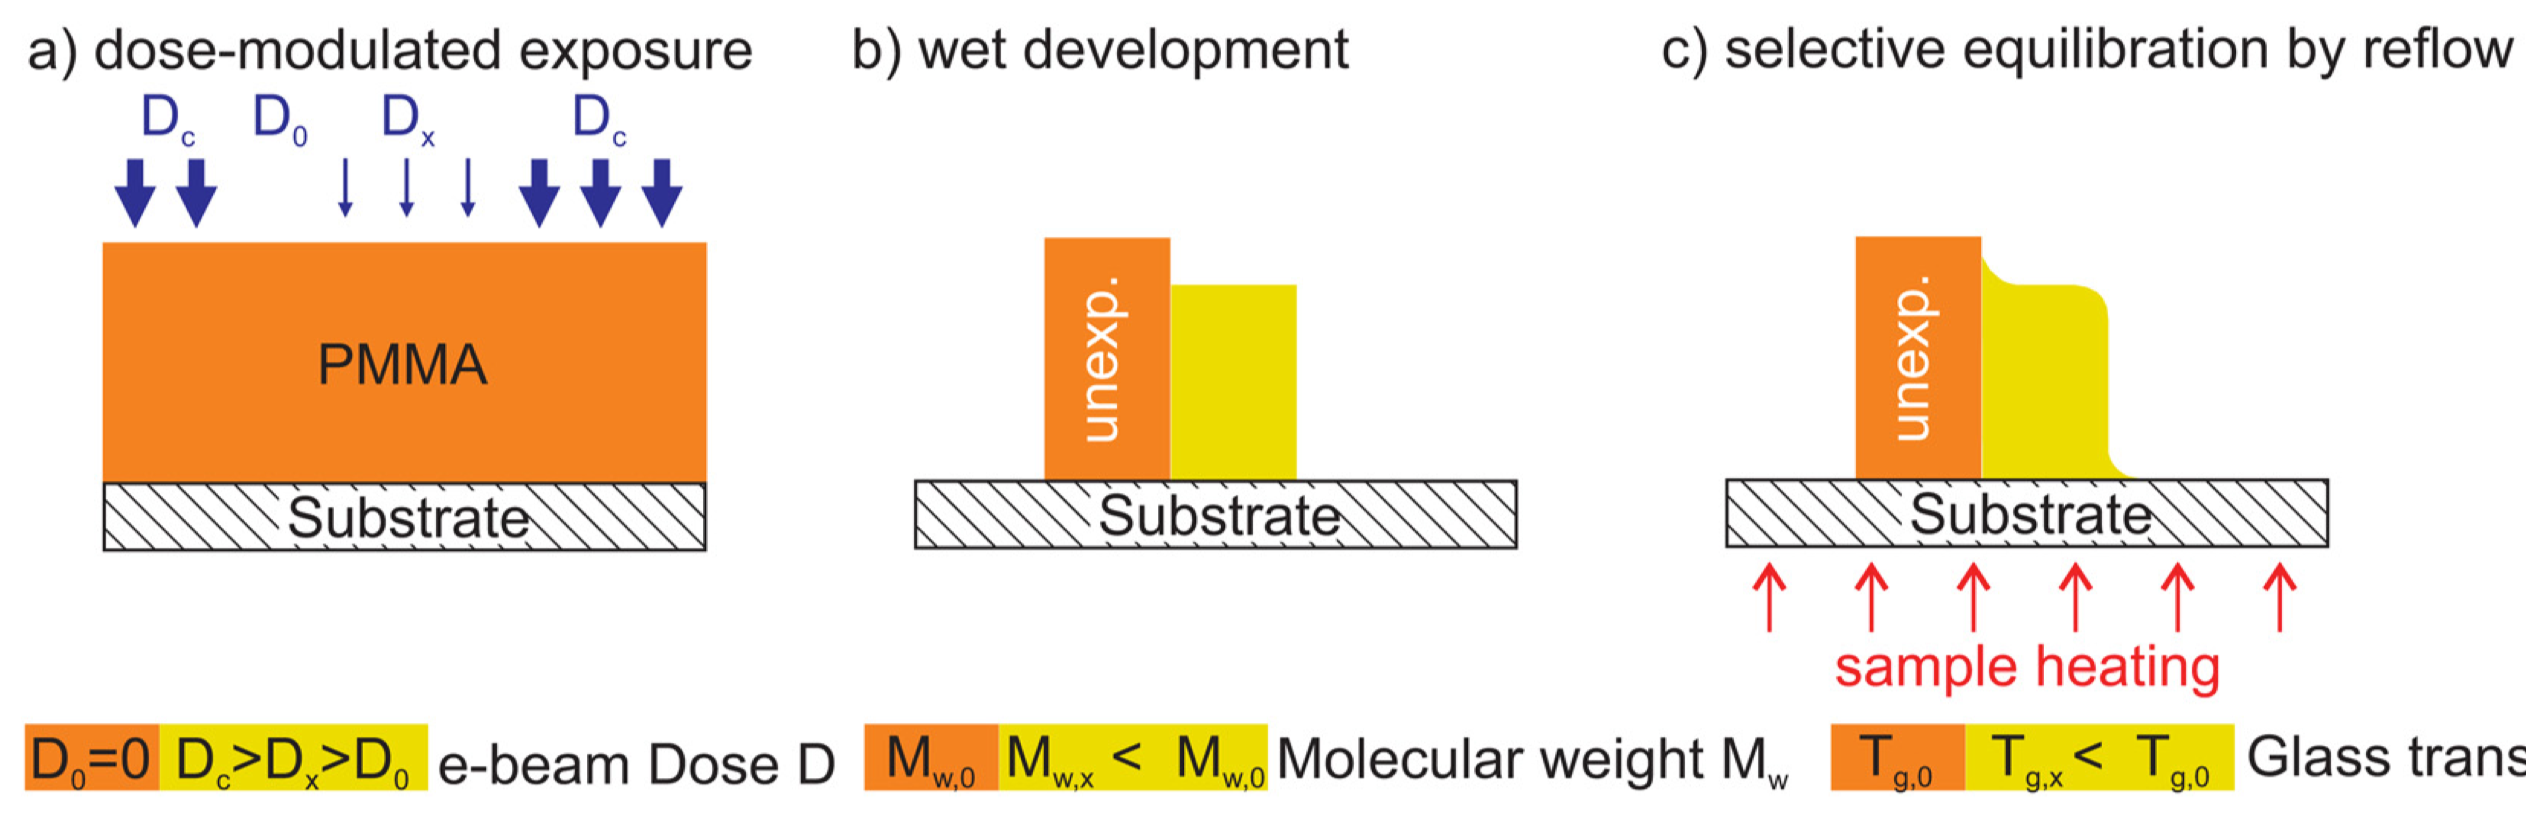
\includegraphics[width=.95\linewidth]{GL_process}
	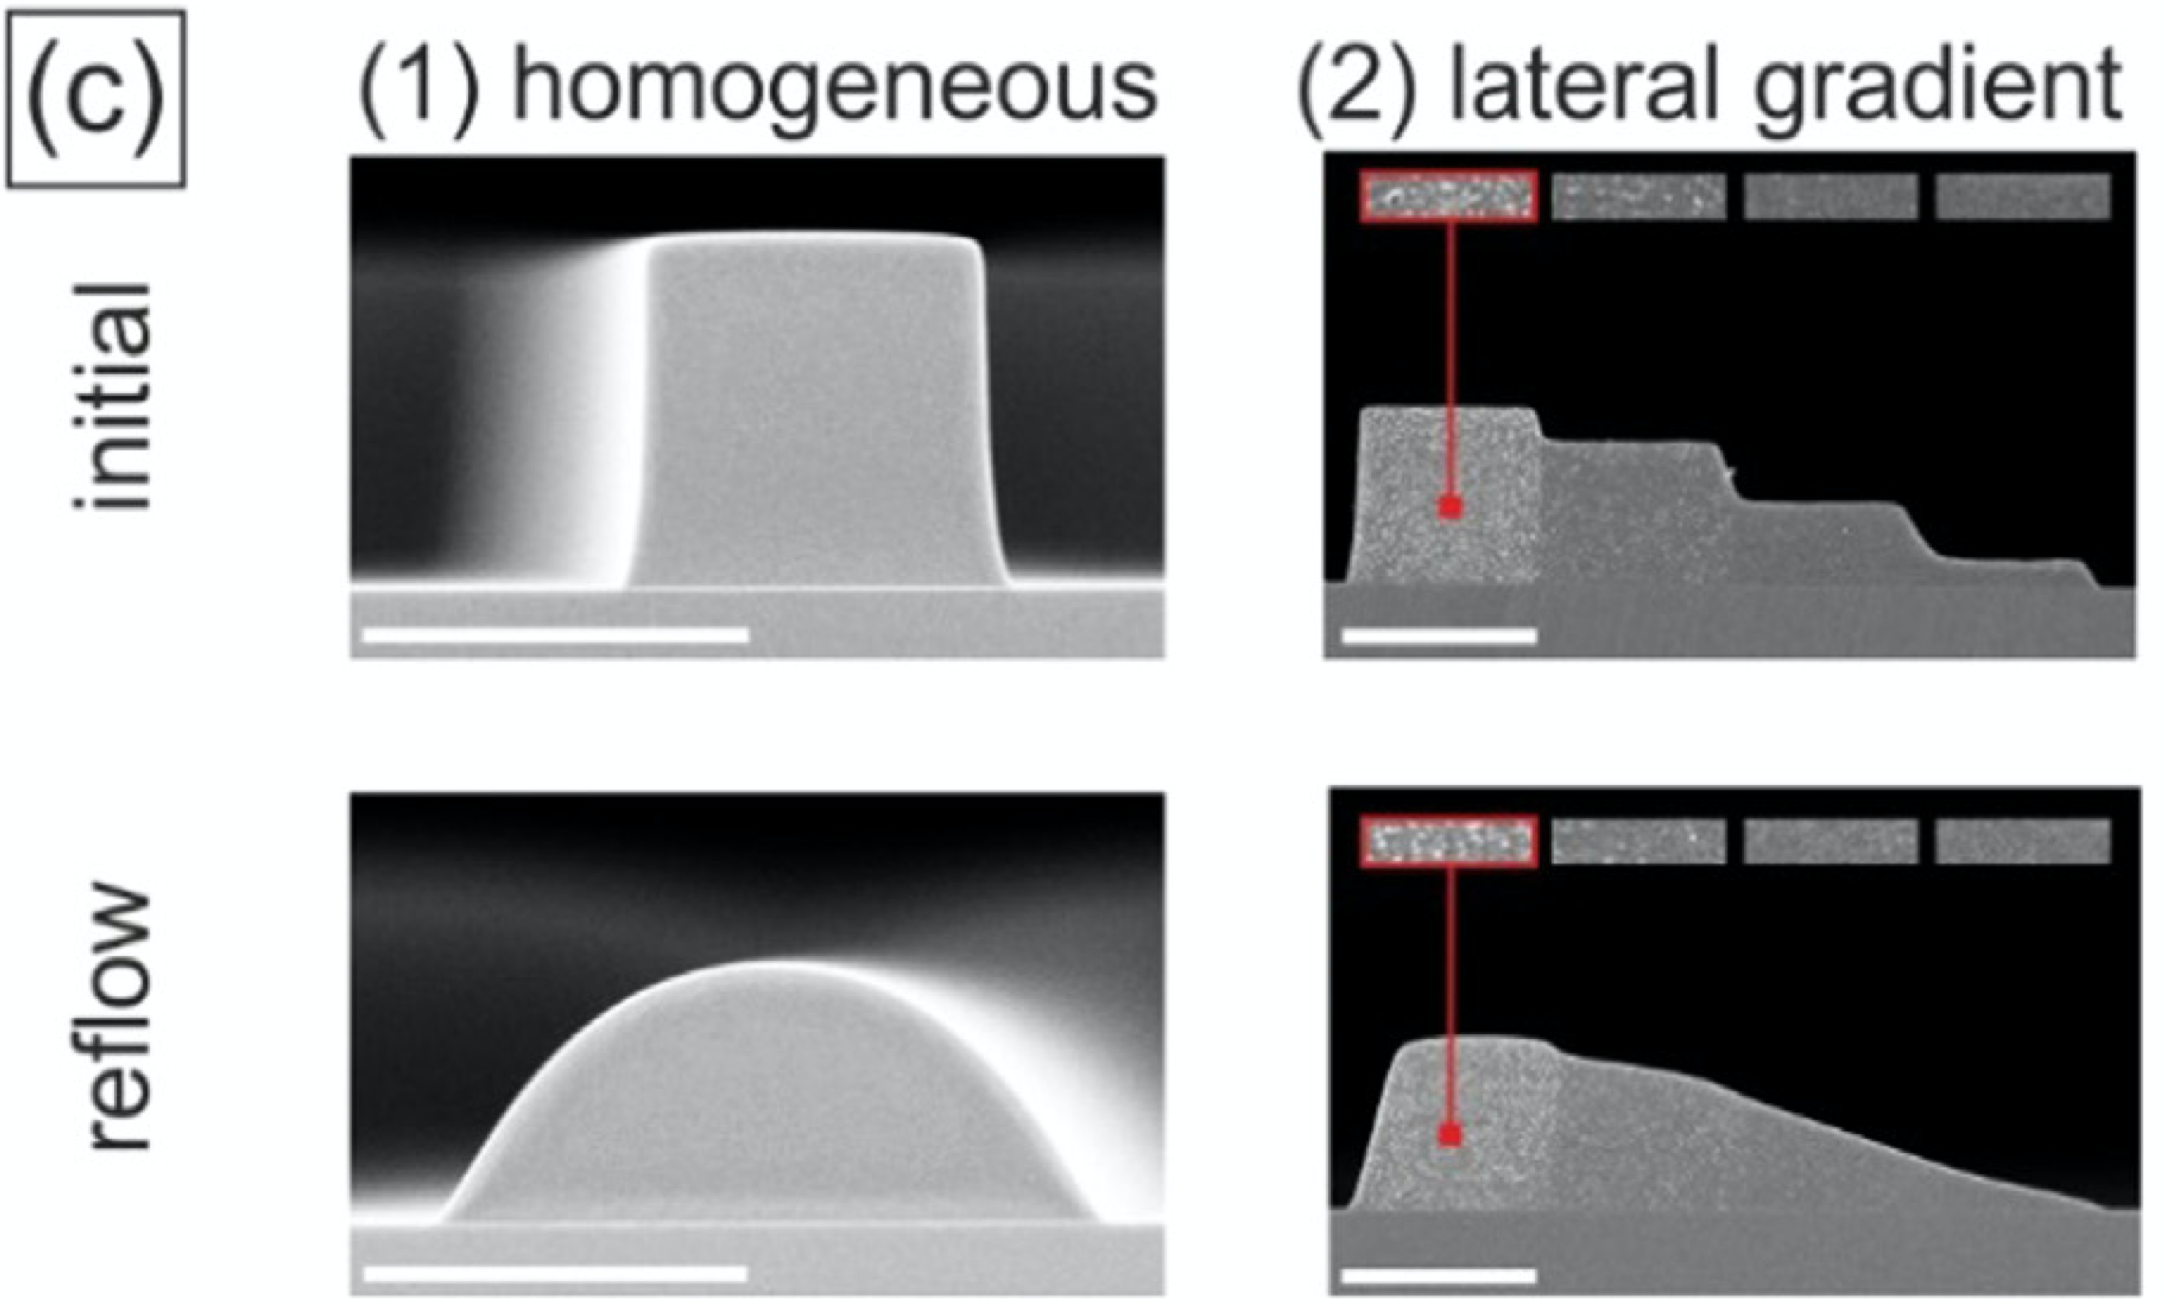
\includegraphics[width=.45\linewidth]{GL_examples}
	\caption{Схематическое изображение процесса ПЛ и примеры структур.}
\end{figure}


\subsection{Сканирующая зондовая литография}

Сканирующая зондовая литография (СЗЛ) включает в себя семейство технологий формирования структур с наноразмерным разрешением. Каждая из технологий основана на применении специального сканирующего зонда для воздействия на поверхность образца, приводящего к локальным изменениям поверхности. В зависимости от природы воздействия зонда на поверхность можно выделить следующие основные виды СЗЛ:
\begin{itemize}
	\item механическая, в которой изменение поверхности образца происходит в результате механического воздействия зонда ~\cite{SPL_mechanical};
	\item  термохимическая, в которой воздействие нагретого зонда на образец приводит к термической активации различных химических реакций в нем~\cite{SPL_termochemical};
	\item СЗЛ с приложением напряжения, при которой высокая напряженность электростатического поля в области зонда приводит к разложению молекул жидкости~\cite{SPL_bias_liquid} или газа~\cite{SPL_bias_gas}, окружающего образец, и локальному отложению материала на образце;
	\item окислительная СЗЛ, основанная на модификации поверхности путем ее локального окисления~\cite{SPL_oxidation};
	\item перьевая СЗЛ, в которой сканирующий зонд используется для нанесения на поверхность образца органических, полимерных или коллоидных наночернил~\cite{SPL_dip_pen_1, SPL_dip_pen_2}
\end{itemize}

Поскольку сканирующий зонд воздействует только на поверхность образца, этот метод может быть использован только для послойного формирования рельефа (в отличие от, например, ДЛЛ). Однако, высокое разрешение этой технологии и возможность ее реализации с использованием различных материалов обеспечили ей широкое применение. При этом, как и ДЛЛ, производительность сканирующей зондовой литографии крайне низка.

\begin{narrowfig}{SPL}{SPL}
	Диаграмма, отображающая различные реализации метода СЗЛ.
\end{narrowfig}


\section{Методы моделирования}

\subsection{Моделирование на основе кинетической теории транспорта}
Моделирование на основе кинетической теории транспорта заключается в решении кинетического уравнения Больцмана, описывающего распространение электронов в структуре. Этот метод успешно применяется для моделирования электронного пучка в планарных структурах, состоящих из небольшого количества слоев~\cite{Stepanova_2006, Stepanova_2010}. Для задач с более сложной геометрией необходимо введение дополнительных граничных условий, что значительно усложняет расчет.

\subsubsection{Определение распределения электронов по глубине}
В большинстве случаев для упрощения расчетов, рассматривается точечный пучок электронов, направленный под прямым углом к поверхности (вдоль оси $z$). Распространение электронов в веществе по глубине может быть описано функцией распределения $f(z, E, \cos \theta_v)$, где z , E – глубина проникновения электрона в образец и его энергия, z – угол между скоростью электрона и осью z . В этом случае уравнение Больцмана принимает вид~\cite{ME_rev_60}:
\begin{equation} \label{eq:Boltzman_1}
	\frac{d E}{d s} \frac{\partial f}{\partial E}+\cos \theta_v \frac{\partial f}{\partial z}=\frac{1}{\Lambda} \int w(\cos \gamma)\left[f\left(\cos \theta_{v^{\prime}}\right)-f\left(\cos \theta_v\right)\right] d \Omega_\gamma,
\end{equation}
где $\frac{dE}{ds}$ -- потери энергии на единицу длины пути, $\Lambda$ –- длина свободного пробега при упругом рассеянии, $v$ и $v^{\prime}$ -- скорости до и после рассеяния, соответственно, $w(\cos \gamma)$ -- нормированное дифференциальное сечение упругого рассеяния на угол $\gamma$:
\begin{equation} \label{eq:Boltzman_2}
	w(\cos \gamma)=\frac{1}{\sigma_{\mathrm{el}}} \frac{d \sigma}{d \Omega_\gamma}
\end{equation}

Уравнение \ref{eq:Boltzman_1} может быть решено в диффузионном приближении~\cite{ME_rev_61}, применимом в диапазоне энергий, характерных для электронно-лучевой литографии. Для этого функция распределения электронов раскладывается по полиномам Лежандра $P(\cos \theta)$:
\begin{equation} \label{eq:Boltzman_3}
	f\left(z, E, \cos \theta_v\right)=\sum_0^{\infty} C_n(z, E) P_n\left(\cos \theta_n\right)
\end{equation}

Подстановка \ref{eq:Boltzman_3} в \ref{eq:Boltzman_1} приводит к разностной дифференциальной схеме для коэффициентов $C_n$:
\begin{equation} \label{eq:Boltzman_4}
	\left(\frac{d E}{d s}\right) \frac{\partial C_n}{\partial E}+\frac{n}{2 n-1} \frac{\partial C_{n-1}}{\partial z}+\frac{n+1}{2 n+3} \frac{\partial C_{n+1}}{\partial z}=-\frac{1}{\lambda_n} C_n,
\end{equation}
где
\begin{equation} \label{eq:Boltzman_5}
	\frac{1}{\lambda_n}=\frac{1}{\Lambda} \int\left[1-P_n(\cos \gamma)\right] W(\cos \gamma) d \Omega_\gamma
\end{equation}

Коэффициенты $C_0$ и $C_1$ пропорциональны плотности вероятности и проекции плотности потока вероятности на ось $z$, соответственно:
\begin{equation} \label{eq:Boltzman_6}
	\begin{gathered}
		\rho(z, E)=\int f\left(z, E, \cos \theta_v\right) d \Omega_v=4 \pi C_0(z, E), \\
		J_z(z, E)=\int v \cos \theta_v f\left(z, E, \cos \theta_v\right) d \Omega_v=\frac{4 \pi}{3} v C_1(z, E).
	\end{gathered}
\end{equation}

Точное решение \ref{eq:Boltzman_1} возможно при отбрасывании в  коэффициентов $C_n$ с \break $n>1$, соответствующими турбулентному движению. При этом \ref{eq:Boltzman_4} приводит к уравнению диффузии:
\begin{equation} \label{eq:Boltzman_7}
	\frac{\partial}{\partial E} \rho(z, E)=a(E) \frac{\partial^2}{\partial z^2} \rho(z, E), a(E)=\left(\frac{d E}{d s}\right)^{-1} \frac{\lambda_1}{3} .
\end{equation}
Его решение:
\begin{equation} \label{eq:Boltzman_8}
	\rho(z, E)=\frac{1}{\sqrt{\pi} \sigma(E)} \exp \left(-\frac{z^2}{4 \sigma^2(E)}\right)\left\{1-\frac{\sqrt{\pi} \sigma(E)}{\Delta \lambda_1\left(E_0\right)} \exp \left(\varsigma^2\right) \operatorname{erfc}\left(\varsigma^2\right)\right\},
\end{equation}
где
\begin{equation} \label{eq:Boltzman_9}
	\zeta=\frac{z}{2 \sigma(E)}+\frac{\sigma(E)}{\Delta \lambda_1\left(E_0\right)}, \quad \sigma^2=\int a(E) d E, \quad \Delta=0.71
\end{equation}

Для описания функции распределения электронов в системе, состоящей из нескольких слоев, решение для предыдущего слоя используется как граничное условие для уравнения диффузии в новом слое.


\subsubsection{Определение латерального распределения электронов}
Латеральное распределение электронов описывается функцией плотности вероятности $\rho(r, z, E)$, определяющей вероятность нахождения электрона с энергией E в кольце радиуса $r$, имеющем объем $2 \pi r dr dz$ и расположенном параллельно поверхности резиста на глубине $z$. Для определения продольного распределения электронов, необходимо решение уравнения Больцмана в более общем виде, чем \ref{eq:Boltzman_1}~\cite{ME_rev_63}, и при этом отдельно учитывается вклад от электронов, рассеянных на малые углы (индекс $f$), обратного рассеянных электронов (индексы $bd$ и $bs$) и вторичных электронов (индекс $s$)~\cite{ME_rev_64}:
\begin{equation} \label{eq:Boltzman_10}
	\rho(r, z, E)=\rho(z, E)\left[\rho_f(r \mid z, E)+\rho_{b d}(r \mid z, E)\right]+\rho_{b s}(r, z, E)+\rho_s(r, z, E).
\end{equation}
Здесь выражения вида $\rho(r|z,E)$ означают плотность вероятности при известных значениях z и E. Слагаемое $\rho_f(r|z,E)$ описывает вклад в продольное уширение пучка за счет малого количества актов рассеяния первичных электронов на малые углы в слое резиста:
\begin{equation} \label{eq:Boltzman_11}
	\rho_f(r \mid z, E)=\frac{3 \lambda_1}{2 \pi z^3} \exp \left(-\frac{3 \lambda_1 r^2}{2 z^3}\right)
\end{equation}
где $\lambda_1$ определяется из соотношения \ref{eq:Boltzman_5}.

Обратное рассеяние электронов происходит за счет малого количества актов рассеяния на большие углы вблизи границы резиста с подложкой ($\rho_{bs}$), либо за счет диффузии электронов в структуре ($\rho_{bd}$):
\begin{equation} \label{eq:Boltzman_12}
	\begin{gathered}
		\rho_{b s}(r, z, E)=\frac{1}{\pi} \int_z^{z_d} \beta(1+\beta) \rho\left(z^{\prime}, E\right) \frac{z^{\prime}-z}{R} \frac{d z^{\prime} / \Lambda}{\left[(1+\beta) R+z^{\prime}-z\right]^2}, \\
		\rho_{b d}(r \mid z, E)=\frac{A^2}{3} \int_{z_d}^{z_{\max }}\left(\frac{1}{4 \pi \sigma_b^2}\right)^{3 / 2} \exp \left(-\frac{R^2}{4 \sigma_b^2}\right) \frac{z^{\prime}-z}{z_{\max }-z_d} d z^{\prime},\\
		R=\sqrt{r^2+\left(z-z^{\prime}\right)^2}, \\ \sigma_b^2=\int_{E\left(z^{\prime}\right)}^{E(z)} a\left(E^{\prime}\right) d E^{\prime},
	\end{gathered}
\end{equation}
где $\beta$ -- параметр экранирования в формуле Резерфорда для дифференциального сечения упругого рассеяния, $\Lambda$ -- длина свободного пробега для упругого рассеяния, a $a(E)$ – коэффициент диффузии \ref{eq:Boltzman_7}, $E(z)$ , $E(z^\prime)$ – средние энергии электрона, получаемые за счет интегрировании функции $Ef(z, E, \cos \theta_v )$. Параметр z d выражает максимальную глубину проникновения электронов, рассеивающихся на большие углы вблизи границы резиста с подложкой, и его значение выбирается исходя из моделирования методом Монте-Карло. Значения параметров $z_max$ и $A$, определяющих максимальную глубину, на которой могут находиться обратно отраженные электроны и коэффициент обратного отражения электронов соответственно, также выбираются исходя из соответствия результатам Монте-Карло моделирования. Например, для слоя полиметилметакрилата (ПММА) толщиной 0.5 мкм на кремниевой подложке выбираются следующие значения этих параметров: $z_d$ = 0.83 мкм, $z_{max}$ = 8.5 мкм, $A$ = 0.19.

Вклад вторичных электронов в уширение пучка описывается плотностью вероятности вторичных электронов:
\begin{equation} \label{eq:Boltzman_13_0}
	\rho_s(r, z, E)=\int_{2 E}^{E_0} d E^{\prime} P_{inel}\left(E^{\prime}\right) \Phi\left(E, E^{\prime}\right) \int d^3 \vec{r}^{\prime} \frac{1}{8 \pi S^3(E)} \exp \left(\frac{-\left|\vec{r}-\vec{r}^{\prime}\right|}{S(E)}\right) \rho\left(r^{\prime}, z, E^{\prime}\right).
\end{equation}
Здесь $E_0$ -- начальная энергия электронов, $P_{inel}$ вероятность неупругого рассеяния, в котором возникает вторичный электрон, определяемая из выражений для сечения упругого и неупругого рассеяния ($\sigma_{el}$ и $\sigma_{inel}$, соответственно):
\begin{equation} \label{eq:Boltzman_13}
	P_{inel}=\frac{\sigma_{inel}}{\sigma_{el}+\sigma_{inel}},
\end{equation}
Функция $\Phi\left(E, E^{\prime}\right)$ представляет дифференциальное сечение неупругого рассеяния, нормированное на полное сечение неупругого рассеяния, $S(E)$ -- максимальная глубина проникновения электронов, выражающаяся через потери энергии на единицу пути:
\begin{equation} \label{eq:Boltzman_14}
	S(E)=\int_{E_0}^{E_{\min }} d E\left(\frac{d E}{d s}\right)^{-1}
\end{equation}

Одним из наиболее важных результатов моделирования является распределение энергии, выделенной в резисте. Плотность выделенной энергии в расчете на один электрон $I(r,z)$ может быть получена за счет интегрирования произведения плотности вероятности и функции потерь энергии~\cite{ME_rev_64}.


\subsection{Моделирование методом Монте-Карло}
При моделировании методом Монте-Карло для каждого электрона из пучка рассчитывается его траектория в структуре. Параметры траектории и потери энергии электрона определяются из дифференциальных сечений упругих и неупругих процессов с использованием случайных чисел из равномерного распределения на промежутке [0, 1). Данный метод требует больших вычислительных мощностей, но при этом его сложность практически не зависит от формы структуры и количества входящих в нее материалов. Также, в отличие от моделирования на основе кинетической теории транспорта, алгоритм расчета траектории электрона в структуре методом Монте-Карло позволяет воспроизвести стохастичность процессов рассеяния.

\subsubsection{Определение длины пробега электрона}
Путем интегрирования дифференциальных сечений вычисляются значения полных сечений упругого и неупругого рассеяния электронов в веществе:
\begin{equation} \label{eq:MC_1}
	\sigma_{el/inel}(E) = \int_Q \frac{d \sigma_{el/inel}(E, q)}{dq} dq
\end{equation}
где индекс <<$$el/inel$$>> означает тип рассеяния -- упругое рассеяние или неупругое, соответственно. Дифференциальные сечения рассеяния зависят как от энергии налетающего электрона, так и от второй переменной, которая здесь называется $q$. Для упругого рассеяния это полярный угол рассеяния $\theta$ , для неупругого -- энергия $\Delta E$, передаваемая налетающим электроном среде. Интегрирование в формуле \ref{eq:MC_1} производится по области всех возможных значений $q$. Далее определяется полное сечение рассеяния на атомах всех типов:
\begin{equation} \label{eq:MC_3}
	\lambda_{el/inel}(E)=\left(n \sigma_{el/inel}(E)\right)^{-1},
\end{equation}
длина свободного пробега определяется по формуле:
\begin{equation} \label{eq:MC_4}
	\lambda^{-1}(E) = \lambda_{el}^{-1}(E)+\lambda_{inel}^{-1}(E).
\end{equation}

Вероятность того, что на промежутке пути длиной s не произойдет рассеяния, равна~\cite{ME_rev_49}:
\begin{equation} \label{eq:MC_5}
	p(s) = \lambda(E)^{-1} \exp \left(-\frac{s}{\lambda(E)}\right)
\end{equation}

При Монте-Карло моделировании длина пробега электрона может быть определена по формуле:
\begin{equation} \label{eq:MC_6}
	s = -\lambda(E) \ln \left(\xi_1\right)
\end{equation}
где $\xi_1$ случайное число из промежутка [0, 1). Если пробег электрона начинается и заканчивается в слоях, состоящих из разного вещества (например, моделирование проводится для системы из $m$ слоев с толщинами $s_1$, $s_2$, ..., $s_m$ и длинами свободного пробега электронов $\lambda_1$, $\lambda_2$, ..., $\lambda_m$), длина пробега электрона s должна быть пересчитана с условием пересечения границы между слоями. Например, она может быть вычислена как верхний предел интеграла в формуле~\cite{Han_2002}:
\begin{equation} \label{eq:MC_7}
	\ln \left(\xi_1\right)=-\frac{s_1}{\lambda_1}-\frac{s_2}{\lambda_2} \ldots+\int_{s_k}^s-\frac{d u}{\lambda_k}
\end{equation}
где $k \leq m$.

\subsubsection{Определение типа взаимодействия и атома}
Далее на основе вероятностей упругого и неупругого рассеяния
\begin{equation} \label{eq:MC_8}
	p_{el/inel}=\sigma_{el/inel} /\left(\sigma_{el}+\sigma_{inel} \right)
\end{equation}
определяется тип взаимодействия (упругое или неупругое рассеяние), в котором электрон примет участие после прохождения пути $s$:
\begin{equation} \label{eq:MC_9}
	\begin{aligned}
		\xi_2 < p_{el} & \Rightarrow \text{упругое рассеяние} \\
		\xi_2 > p_{el} & \Rightarrow \text{неупругое рассеяние}
	\end{aligned}
\end{equation}
где $\xi_2$ -- новое случайное число из промежутка [0, 1).

\subsubsection{Определение нового направления электрона и потерь энергии}
В случае упругого рассеяния определяется новое направление рассеянного электрона, для чего используются случайные числа -- $\xi_3$ и $\xi_4$. Азимутальный угол рассеяния $\varphi$ считается равномерно распределенным на промежутке [0, 2$\pi$) и определяется выражением:
\begin{equation} \label{eq:MC_11}
	\phi = 2 \pi \xi_3.
\end{equation}

Полярный угол рассеяния $\theta$ вычисляется на основе дифференциального сечения упругого рассеяния по формуле:
\begin{equation} \label{eq:MC_12}
	\xi_4 = \frac
	{\displaystyle \int_0^\theta \frac{d \sigma}{d \Omega} \sin \vartheta d \vartheta}
	{\displaystyle \int_0^\pi \frac{d \sigma}{d \Omega} \sin \vartheta d \vartheta}.
\end{equation}

При известных углах $n$-ого акта рассеяния $\phi_n$ и $\theta_n$ новое направление движения электрона $\vec{x}_n$ определяется начальным направлением движения электронов в пучке $x_0$ (часто выражаемом вектором $(0,0,1)$) и комбинацией матриц поворота~\cite{rotation_matrices}:
\begin{equation} \label{eq:MC_13}
	\vec{x}_n=O_n^T \vec{x}_0, \quad O_n=W_n O_{n-1},
\end{equation}
\begin{equation} \label{eq:MC_14}
	W_n=\left(\begin{array}{ccc}
		\cos \varphi_n & \sin \varphi_n & 0 \\
		-\sin \varphi_n \cos \theta_n & \cos \varphi_n \sin \theta_n & \sin \theta_n \\
		\sin \varphi_n \sin \theta_n & -\cos \varphi_n \sin \theta_n & \cos \theta_n
	\end{array}\right).
\end{equation}
При этом используются начальные значения $O_{-1} = E$ (единичная матрица) и $\phi_0 = \theta_0 = 0$.

В случае неупругого рассеяния определяются потери энергии. При использовании модели непрерывных потерь энергии, потери энергии на пути $s$, определяемом выражением \ref{eq:MC_6} , вычисляются по формуле:
\begin{equation} \label{eq:MC_15}
	\Delta E=\int_0^s \frac{d E}{d s} d s \approx \frac{d E}{d s} s
\end{equation}

При использовании модели дискретных потерь энергии, потери энергии $\Delta E$ определяются с помощью случайного числа $\xi_5$:
\begin{equation} \label{eq:MC_16}
	\xi_5 = \frac
	{\displaystyle \int_{E_{\min }}^{\Delta E} \frac{d \sigma}{d\left(\Delta E^{\prime}\right)} d\left(\Delta E^{\prime}\right)}
	{\displaystyle \int_{E_{\min }}^{E_{\max }} \frac{d \sigma}{d\left(\Delta E^{\prime}\right)} d\left(\Delta E^{\prime}\right)},
\end{equation}
где дифференциальные сечения неупругого рассеяния $\frac{d \sigma}{d \Delta E}$ вычисляются по формуле Гризинского или из диэлектрической функции, а в качестве значений $E_{min}$ и $E_{max}$ выбираются $0$ и $E/2$, соответственно~\cite{Dapor_large_book}. Пример траектории электрона, рассчитываемой по методу Монте-Карло, приведен на рис.~\ref{fig:Monte_Carlo_scheme}.

%\begin{fig}{Monte_Carlo_scheme}{Monte_Carlo_scheme}[]
%	Схематическое изображение траектории электрона в веществе, получаемой при Монте-Карло моделировании при использовании модели непрерывных потерь энергии.
%\end{fig}

\begin{figure}
	\centering
	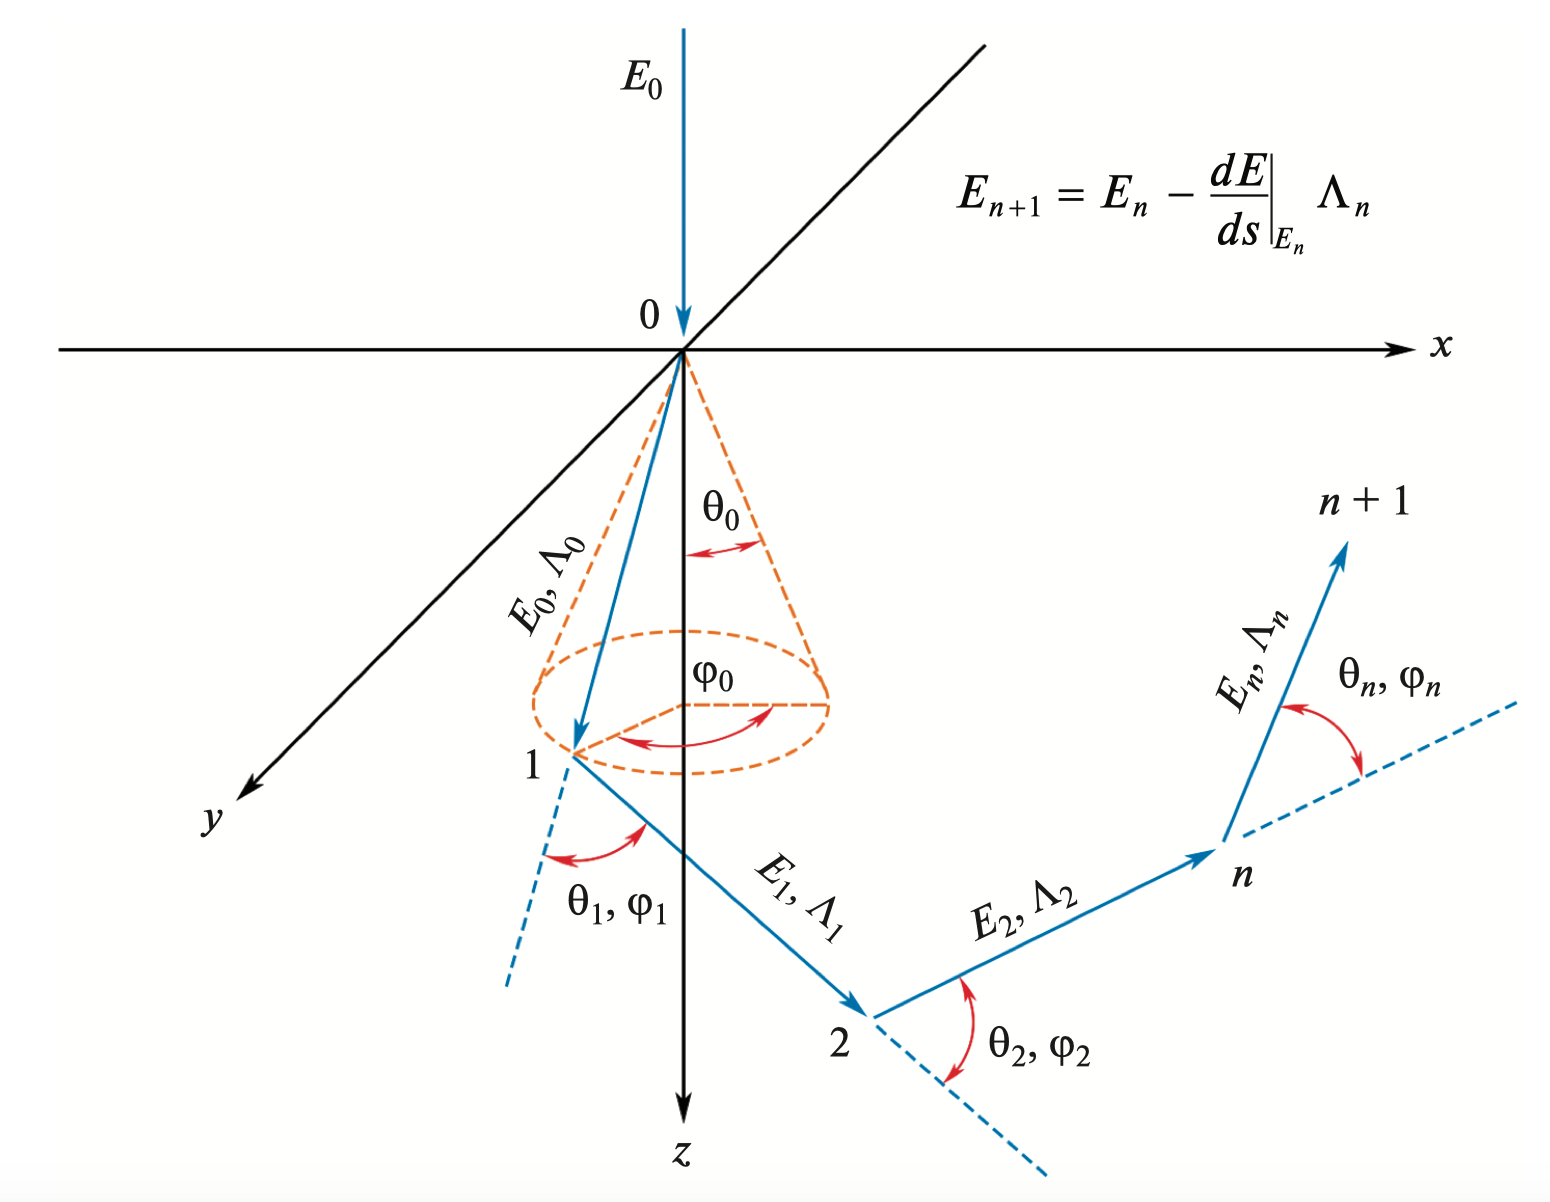
\includegraphics[width=0.6\linewidth]{Monte_Carlo_scheme}
	\caption{Схематическое изображение траектории электрона в веществе, получаемой при Монте-Карло моделировании при использовании модели непрерывных потерь энергии.}
	\label{fig:Monte_Carlo_scheme}
\end{figure}

%В случае использования формулы Гризинского, $E_{min}$ принимается равным энергии связи нужной оболочки, $E_{max}$ -- энергии налетающего электрона $E$. В случае использования диэлектрической функции, $E_{min} = 0$, $E_{max} = E - E_F$, где $E_F$ -- энергия Ферми~\cite{Shimizu_review}. 


\section{Модели взаимодействия электронного излучения с веществом}

\subsection{Модели упругого рассеяния электронов в веществе}
Упругое рассеяние происходит в основном в результате столкновения высокоэнергетических электронов с ядрами атомов, частично экранированными связанными электронами. При этом изменяется направление движения электрона, а его энергия остается практически неизменной. Азимутальный угол рассеяния $\phi$ распределен равномерно в промежутке (0$^\circ$, 360$^\circ$), полярный угол рассеяния $\theta$ распределен в промежутке (0$^\circ$ до 180$^\circ$) со средним значением 5$^\circ$-10$^\circ$.

Основной характеристикой упругого рассеяния электрона на атомах вещества является дифференциальное сечение рассеяния $\frac{d \sigma}{d \Omega}$, определяемое как отношение числа частиц, рассеянных мишенью в элемент телесного угла $d \Omega = d \varphi \sin \theta d \theta$ за единицу времени к плотности потока налетающих частиц. Интеграл от дифференциального сечения по полному телесному углу определяется как полное сечение упругого рассеяния:
\begin{equation} \label{eq:models_1}
	\sigma_{el}=2 \pi \int_0^\pi \frac{d \sigma}{d \Omega} \sin \theta d \theta.
\end{equation}

\subsubsection{Формула Резерфорда}
Для определения дифференциального сечения упругого рассеяния электронов на атомах вещества можно воспользоваться формулой Резерфорда~\cite{Dapor_large_book}:
\begin{equation} \label{eq:models_3}
	\frac{d \sigma_R}{d \Omega}=\frac{Z^2 e^4}{4 E^2(1-\cos \theta+2 \beta)^2},
\end{equation}
где $Z$ -- зарядовое число атомов вещества, $e$ -- заряд электрона, $E$ -- энергия налетающего электрона, $\beta$ -- параметр экранирования поля ядра атома-мишени атомными электронами. Формула Резерфорда хорошо описывает сечения упругого рассеяния электронов на легких атомах, однако, ее точность снижается с ростом зарядового числа атомов, особенно, в области низких энергий электронов (<1 кэВ) (рис. 1) [7–10].

\subsubsection{Моттовские сечения}
Более точные значения сечений упругого рассеяния (моттовские сечения) могут быть получены за счет решения уравнения Дирака для рассеяния релятивистского электрона в центральном статическом поле атома-мишени~\cite{Czyzewski_mott_cs}. В этом подходе дифференциальное сечение упругого рассеяния задается формулой:
\begin{equation}
	\frac{d \sigma_{e l}}{d \Omega}=|f(\theta)|^2+|g(\theta)|^2,
\end{equation}
где $f(\theta)$ и $g(\theta)$ -- амплитуды рассеяния, соответствующими параллельному и антипараллельному направлению спина электрона относительно его направления движения, соответственно, и определяемые выражениями:
\begin{equation}
	\begin{aligned}
		&f(\theta)=\frac{1}{2 i K} \sum_{l=0}^{\infty}\left\{(l+1)\left[\exp \left(2 i \delta_l^{-1}\right)-1\right]+l\left[\exp \left(2 i \delta_l^{+}\right)-1\right]\right\} P_l(\cos \theta) \\
		&g(\theta)=\frac{1}{2 i K} \sum_{l=0}^{\infty}\left[-\exp \left(2 i \delta_l^{-}\right)+\exp \left(2 i \delta_l^{+}\right)\right] P_l^1(\cos \theta).
	\end{aligned}
\end{equation}
Здесь $k$ -- волновое число налетающего релятивистского электрона, $P_l(\cos \theta)$ и $P_l^1 (\cos \theta)$ -- полиномы Лежандра и присоединенные полиномы Лежандра, соответственно, фазовые сдвиги сферических волн, рассчитываемые по формуле:
\begin{equation}
	\tan \left(\eta_l\right)=\frac{K j_{l+1}(K r)-j_l(K r)\left[(W+1) \tan \phi_l^{\pm}+\left(1+l+k^{\pm}\right) / r\right]}{K n_{l+1}(K r)-n_l(K r)\left[(W+1) \tan \phi_l^{\pm}+\left(1+l+k^{\pm}\right) / r\right]},
\end{equation}
где $K^2 = W^2 - 1$ , $W$ -- полная энергия электрона в единицах $mc^2$, $r$ -- расстояние до рассеивающего центра в единицах $h/2 \pi mc$. 
Индексы <<+>> и <<0>> обозначают параллельное и антипараллельное направление спина, соответственно:
\begin{equation}
	\begin{aligned}
		&+: k^{+}=-l-1, \quad & j=l+1 / 2, \\
		&-: k^{-}=l, \quad & j=l-1 / 2 .
	\end{aligned}
\end{equation}

При этом $\phi_l^\pm$ -- предел функции $\phi_l^\pm (r)$ (при $r \rightarrow \infty$), которая находится путем численного интегрирования уравнения Дирака:
\begin{equation}
	\frac{d \phi_l^{\pm}(r)}{d r}=\frac{k^{\pm}}{r} \sin \left[2 \phi_l^{\pm}(r)\right]-\cos \left[2 \phi_l^{\pm}(r)\right]+W-V(r)
\end{equation}
где $V(r)$ -- рассеивающий потенциал.


\subsection{Модели неупругого рассеяния электронов в веществе}
Квазиупругие и неупругие процессы включают в себя все процессы взаимодействия между налетающим электроном и веществом мишени, в которых электрон теряет свою энергию. При этом также происходит изменение направления движения электрона, и полярный угол рассеяния $\theta$ задается выражением~\cite{Ciappa_2010}:
\begin{equation}
	\sin ^2 \theta=\frac{\hbar \omega}{E},
\end{equation}
где $E$ -- энергия электрона до акта рассеяния, $\hbar \omega$ -- потери энергии. В моделях неупругого рассеяния часто рассматривается взаимодействие налетающего электрона с веществом мишени в целом, и для описания такого взаимодействия используется обратная длина свободного пробега $\lambda_{inel}^{-1}(E)$, связанная с сечением неупругого рассеяния формулой:
\begin{equation}
	\lambda_{\text {inel }}^{-1}(E)=n \sigma(E),
\end{equation}
где $n$ -- концентрация рассеивающих центров в веществе.


\subsubsection{Модель непрерывных потерь энергии}
Исторически первые подходы к описанию потерь энергии электрона в веществе основывались на формуле Бете~\cite{Bethe}:
\begin{equation}
	-\left(\frac{d E}{d s}\right)_{\text {Bethe }}=2 \pi e^4 N_{\mathrm{A}} \frac{\rho}{Z} \frac{1}{E} \ln \left(\frac{1.66 E}{J}\right),
\end{equation}
где $N_A$ -- число Авогадро, $\rho$ -- плотность вещества, $Z$ -- его порядковый номер, соответственно, $e$ и $E$ -- заряд и энергия движущегося в веществе электрона, соответственно. Средний потенциал ионизации $J$ определяется экспериментально или вычисляется на основе порядкового номером атомов вещества~\cite{Dapor_large_book}:
\begin{equation}
	\frac{J}{Z}=9.76+58.8 Z^{-1.19}
\end{equation}
Формула Бете с высокой точностью описывает потери энергии в области высоких энергий налетающего электрона ($E \gg J$). Однако, при приближении энергии налетающего электрона к среднему потенциалу ионизации точность формулы снижается, а в области потери энергии, рассчитываемые по ней, становятся отрицательными. Существуют модификации формулы Бете, позволяющие использовать ее в области низких энергий~\cite{Bethe_corrected}, в которых потери энергии описываются степенной функцией при $E \rightarrow 0$:
\begin{equation}
	-\frac{dE}{ds} \propto \frac{1}{\sqrt{E}}
\end{equation}
В таком виде формула Бете может быть использована, например, для оценки количества обратно отраженных и вторичных электронов, что дает правдоподобные результаты~\cite{Bethe_corr_2ndary_e}. Однако, неограниченный рост потерь энергии при $E \rightarrow 0$ противоречит эмпирическим данным, согласно которым при уменьшении энергии электрона, его потери энергии достигают максимума при энергии в несколько сотен электрон вольт, затем стремятся к нулю~\cite{Shimizu_Review}.


\subsubsection{Модель дискретных потерь энергии}
В современных моделях неупругого рассеяния потери энергии электрона в веществе сводятся к дискретным процессам. В них, аналогично случаю с упругим рассеянием, вводится дифференциальная обратная длина свободного пробега $\frac{d \lambda_{inel}^{-1}}{d \hbar \omega}(E, \hbar \omega)$, позволяющая определить обратную длину свободного пробега по формуле~\cite{Dapor_large_book}:
\begin{equation}
	\lambda_{inel}^{-1}(E)=\int_0^{E / 2} \frac{d \lambda_{\text {inel }}^{-1}(E, \hbar \omega)}{d \hbar \omega} d \hbar \omega,
\end{equation}
а также потери энергии электрона на единицу длины пути $\frac{dE}{ds}$ по формуле:
\begin{equation}
	\frac{dE}{ds}(E) = \int_0^{E / 2} \frac{d \lambda_{\text {inel }}^{-1}(E, \hbar \omega)}{d \hbar \omega} \hbar \omega d \hbar \omega.
\end{equation}

Потери энергии $\hbar \omega$ при неупругом рассеянии также определяются на основе функции $\frac{d \lambda_{inel}^{-1}}{d \hbar \omega}$  методом Монте-Карло~\cite{Ciappa_2010}.

Наиболее распространенный подход к определению дифференциальной обратной длины свободного пробега основана на использовании функции потерь энергии (Energy Loss Function, ELF)~\cite{Dapor_large_book}:
\begin{equation}
	\operatorname{ELF}(q, \omega) \equiv \operatorname{Im}\left[\frac{-1}{\varepsilon(q, \omega)}\right]
\end{equation}
где $\varepsilon(q, \omega)$ -- комплексная диэлектрическая функция, $\vec{q}$ и $\hbar \omega$ -- передаваемые среде импульс и энергия, соответственно. При известной функции потерь энергии дифференциальная обратная длина свободного пробега может быть найдена по формуле:
\begin{equation}
	\frac{d \lambda_{\text {inel }}^{-1}}{d \hbar \omega}=\frac{1}{\pi E a_0} \int_{k_{-}}^{k_{+}} \operatorname{Im}\left[\frac{-1}{\varepsilon(q, \omega)}\right] \frac{d q}{q},
\end{equation}
где
\begin{equation}
	q_{\pm}=\frac{\sqrt{2 m}}{\hbar}(\sqrt{E} \pm \sqrt{E-\hbar \omega}),
\end{equation}
$E$ -- энергия налетающего электрона, m -- масса электрона и $a_0$ -- боровский радиус.

Поскольку функция $\varepsilon(q, \omega)$ может быть найдена из первых принципов только в нескольких идеализированных случаях~\cite{Ritchie_ELF}, часто используется подход на основе оптической функции потерь энергии (Optical Energy Loss Function, OELF), получаемой в пределе $q \rightarrow 0$:
\begin{equation}
	\operatorname{OELF}(\omega) \equiv E L F(0, \omega)=\operatorname{Im}\left[\frac{-1}{\varepsilon(0, \omega)}\right]
\end{equation}

Оптическая функция потерь энергии может быть рассчитана на основе значений коэффициентов преломления ($n$) и поглощения ($k$)~\cite{Dapor_2015_oscillators}:
\begin{equation}
	\operatorname{Im}\left[\frac{-1}{\varepsilon(0, \omega)}\right]=\frac{2 n k}{\left(n^2+k^2\right)^2}
\end{equation}
Коэффициенты n и k табулированы для низких энергий (примерно до 2 кэВ)~\cite{Palik}, для более же высоких энергий они могут быть найдены из компонент атомных факторов рассеяния $f = f_1 + i f_2$ (для молекулярных веществ)~\cite{Henke_photoabs}:
\begin{equation}
	\begin{aligned}
		&n=1-\frac{e^2}{2 \pi m c^2} \lambda^2 N \sum_p x_p f_{1 p}, \\
		&k=\frac{e}{2 \pi m c^2} \lambda^2 N \sum_p x_p f_{2 p}
	\end{aligned}
\end{equation}
где $N$ -- концентрация молекул, содержащих $x_p$ атомов каждого вида, $\lambda$ -- длина волны фотона. Для атомарных веществ оптическая функция потерь энергии может быть найдена непосредственно по формуле:
\begin{equation}
	\operatorname{Im}\left[\frac{-1}{\varepsilon(0, \omega)}\right]=\frac{n_m c \sigma_{p h o t}}{\omega}
\end{equation}
где $n_m$ -- концентрация остовных электронов, $\sigma_phot$ – сечение фотоионизации~\cite{Biggs_cs}. При известной оптической функции потерь энергии поведение функция потерь энергии в области $q > 0$ учитывается с помощью одного из подходов, описанных ниже.


\subsubsection{Аппроксимация функции потерь энергии эмпирической функцией}
Наиболее простым является подход, в котором поведение функции потерь энергии в области $q > 0$ описывается подгоночными функциями $L(x)$ и $S(x)$, что позволяет непосредственно рассчитать обратную длину свободного пробега~\cite{Ashley_LxSx}:
\begin{equation}
	\begin{aligned}
		&\lambda^{-1}(E)=\frac{m e^2}{2 \pi \hbar^2 E} \int_0^{W_{\max }} \operatorname{Im}\left[\frac{-1}{\varepsilon(0, \omega)}\right] L\left(\frac{\hbar \omega}{E}\right) d \hbar \omega, \\
		&L(x)=(1-x) \ln \frac{4}{x}-\frac{7}{4} x+x^{3 / 2}-\frac{33}{32} x^2,
	\end{aligned}
\end{equation}
а также потери энергии на единицу длины пути:
\begin{equation}
	\begin{aligned}
		&\lambda^{-1}(E)=\frac{m e^2}{2 \pi \hbar^2 E} \int_0^{W_{\max }} \operatorname{Im}\left[\frac{-1}{\varepsilon(0, \omega)}\right] L\left(\frac{\hbar \omega}{E}\right) d \hbar \omega, \\
		&L(x)=(1-x) \ln \frac{4}{x}-\frac{7}{4} x+x^{3 / 2}-\frac{33}{32} x^2
	\end{aligned}
\end{equation}


\subsection{Аппроксимация функции потерь энергии суммой осцилляторов Друде}
В данном подходе оптическая функция потерь энергии приближается суммой осцилляторов Друде [77]:
\begin{equation}
	\operatorname{Im}\left[\frac{-1}{\varepsilon(0, \omega)}\right]=\sum_i \frac{A_i \Gamma_i \hbar \omega}{\left[E_i^2-(\hbar \omega)^2\right]^2+\left(\Gamma_i \hbar \omega\right)^2}
\end{equation}
параметры $E_i$, $\Gamma_i$ и $A_i$ которых определяются путем подгонки [68], [78] (см. рисунок 5б, Таблицу 2). Продолжение оптической функции потерь энергии в область осуществляется за счет использования квадратичного закон дисперсии:
\begin{equation}
	E_i(q)=E_i+\frac{\hbar^2 q^2}{2 m}
\end{equation}
что в дальнейшем позволяет построить функцию потерь энергии (см. рисунок 6а)):
\begin{equation}
	\operatorname{Im}\left[\frac{-1}{\varepsilon(q, \omega)}\right]=\sum_i \frac{A_i \Gamma_i \hbar \omega}{\left[\left(E_i+\frac{\hbar^2 q^2}{2 m}\right)^2-(\hbar \omega)^2\right]^2+\left(\Gamma_i \hbar \omega\right)^2},
\end{equation}

\begin{fig}{OLF_Drude}{OLF_Drude}
	Рисунок 5. а) Оптические функции потерь энергии ПММА и Si, б) оптическая функция потерь энергии ПММА, приближенная суммой осцилляторов Друде.
\end{fig}


\subsubsection{Диэлектрическая функция Мермина}
Наиболее точным подходом к построению функции потерь энергии в органических полимерах является подход на основе модели Мермина [62], [81], [82]. В его основе лежит диэлектрическая функция Мермина для столкновительной плазмы:
\begin{equation}
	\varepsilon_M(q, \omega)=1+\frac{(1+i \gamma / \omega)\left[\varepsilon_L(q, \omega+i \gamma)-1\right]}{1+(i \gamma / \omega)\left[\varepsilon_L(q, \omega+i \gamma)-1\right] /\left[\varepsilon_L(q, 0)-1\right]},
\end{equation}
где $\gamma$ -- постоянная затухания, $\varepsilon_L(q, \omega)$ -- диэлектрическая функция Линдхарда [66]:
\begin{equation}
	\varepsilon_L(q, \omega)=1+\frac{\chi^2}{z^2}\left[f_1(u, z)+i f_2(u, z)\right].
\end{equation}
Здесь $u=\omega /\left(q v_F\right)$, $z=q /\left(2 q_F\right)$ и $\chi^2=e^2 /\left(\pi \hbar v_F\right)$, где $v_F$
-- скорость Ферми валентных электронов вещества, $q_F=m v_F / \hbar$. При этом функции $f_1(u, z)$ и $f_2(u, z)$ определяются формулами:
\begin{equation}
	\begin{aligned}
		f_1(u, z) &=\frac{1}{2}+\frac{1}{8 z}[g(z-u)+g(z+u)] \\
		f_2(u, z) &= \begin{cases}\frac{\pi}{2} u, & z+u<1 \\
			\frac{\pi}{8 z}\left[1-(z-u)^2\right], & |z-u|<1<z+u \\
			0, & |z-u|>1\end{cases}
	\end{aligned}
\end{equation}
где
\begin{equation}
	g(x)=\left(1-x^2\right) \ln \left|\frac{1+x}{1-x}\right|
\end{equation}

Как и в предыдущем подходе, функция потерь энергии вещества суммой функций потерь отдельных осцилляторов, и ее построение проводится в два этапа. Сначала оптическая функция потерь энергии вещества подгоняется суммой функций потерь энергии Мермина (осцилляторов Мермина) $q=0$:
\begin{equation}
	\operatorname{Im}\left[\frac{-1}{\varepsilon(0, \omega)}\right]=\sum_i A_i \operatorname{Im}\left[\frac{-1}{\varepsilon_M\left(\omega_i, \gamma_i, q=0, \omega\right)}\right]
\end{equation}
что позволяет получить параметры $A_i$, $\omega_i$ и $\gamma_i$ отдельных осцилляторов. Параметр $\omega_i$ определяет частоту каждого из осцилляторов, что позволяет найти параметр $v_F$, входящий в величины $u$, $z$ и $\chi$, используемые в диэлектрической функции Линдхарда:
\begin{equation}
	\begin{aligned}
		&\omega_i=\sqrt{\frac{4 \pi n_i e^2}{m}} \Rightarrow n_i=\frac{\omega_i^2 m}{4 \pi e^2} \\
		&v_{F_i}=\frac{\hbar}{m}\left(3 \pi^2 n_i\right)^{1 / 3}
	\end{aligned}
\end{equation}
где $n_i$ -- концентрация электронов, соответствующая осциллятору с индексом $i$, $m$ -- масса электрона. Далее на основе параметров $A_i$, $\omega_i$ и $\gamma_i$ составляется функция потерь энергии:
\begin{equation}
	\operatorname{Im}\left[\frac{-1}{\varepsilon(q, \omega)}\right]=\sum_i A_i \operatorname{Im}\left[\frac{-1}{\varepsilon_M\left(\omega_i, \gamma_i, q, \omega\right)}\right]
\end{equation}
и определяется дифференциальная обратная длина свободного пробега.








\subsection{Моделирование слоя полимера}

\subsection{Моделирование электронно-стимулированных разрывов полимерных молекул}

\subsection{Моделирование термической деполимеризации резиста}

\subsection{Моделирование оплавления резиста на основе аналитического подхода}

\subsection{Моделирование оплавления резиста на основе численного подхода}

\subsection{Моделирование нагрева резиста при экспонировании}

\subsection{Модели диффузии мономера в слое полимера}




